% answers.tex —— 2010 年·普通高等学校招生考试·山东卷·文科 · 参考答案与详细解析片段
% 由 tools/generate_projects.py 依来源总账自 2010/2010_数学真题_山东文_试题.md + 2010/2010_数学真题_山东文_解析正文.md + 2010/2010_数学真题_山东文_答案要点.md 生成，勿手改（改源 MD 后重跑）

\begin{gktip}
固定候选 PDF 仅含题面，无答案页；以下解析与结论均由本库独立推导（非官方答案），并按 600 dpi 原页复核题面。原页未印分值，不补。
\end{gktip}

\begin{answer}
\gksolhead{1}{}

\textbf{题目}：

已知全集 $U=\mathbf R$，集合 $M=\{x\mid x^2-4\leqslant0\}$，则 $\complement_UM=$（　）

（A）$\{x\mid -2<x<2\}$

（B）$\{x\mid -2\leqslant x\leqslant2\}$

（C）$\{x\mid x<-2\text{ \text{或} }x>2\}$

（D）$\{x\mid x\leqslant-2\text{ \text{或} }x\geqslant2\}$

\Needspace{4\baselineskip}
\textbf{解析}

\Needspace{5\baselineskip}
由 $x^2-4\leqslant0$ 得 $-2\leqslant x\leqslant2$，故

\nopagebreak[4]
\[M=[-2,2],\qquad \complement_UM=(-\infty,-2)\cup(2,+\infty).\]

即 $\{x\mid x<-2\text{ \text{或} }x>2\}$。

故选 C。

\gkanswer{答案：C。}

\end{answer}
\begin{answer}
\gksolhead{2}{}

\textbf{题目}：

已知 $\dfrac{a+2\mathrm i}{\mathrm i}=b+\mathrm i$（$a,b\in\mathbf R$），其中 $\mathrm i$ 为虚数单位，则 $a+b=$（　）

（A）$-1$

（B）$1$

（C）$2$

（D）$3$

\Needspace{4\baselineskip}
\textbf{解析}

\nopagebreak[4]
\[\frac{a+2\mathrm i}{\mathrm i}=(a+2\mathrm i)(-\mathrm i)=2-a\mathrm i.\]

\Needspace{5\baselineskip}
由 $2-a\mathrm i=b+\mathrm i$ 得 $b=2$，$-a=1$，即 $a=-1$。故

\nopagebreak[4]
\[a+b=1.\]

故选 B。

\gkanswer{答案：B。}

\end{answer}
\begin{answer}
\gksolhead{3}{}

\textbf{题目}：

函数 $f(x)=\log_2(3^x+1)$ 的值域为（　）

（A）$(0,+\infty)$

（B）$[0,+\infty)$

（C）$(1,+\infty)$

（D）$[1,+\infty)$

\Needspace{4\baselineskip}
\textbf{解析}

\Needspace{5\baselineskip}
因为 $3^x>0$，所以 $3^x+1>1$，从而

\nopagebreak[4]
\[f(x)=\log_2(3^x+1)>\log_21=0.\]

当 $x\to-\infty$ 时 $3^x\to0$，$f(x)\to0$；当 $x\to+\infty$ 时 $f(x)\to+\infty$。故值域为 $(0,+\infty)$。

故选 A。

\gkanswer{答案：A。}

\end{answer}
\begin{answer}
\gksolhead{4}{}

\textbf{题目}：

在空间，下列命题正确的是（　）

（A）平行直线的平行投影重合

（B）平行于同一直线的两个平面平行

（C）垂直于同一平面的两个平面平行

（D）垂直于同一平面的两条直线平行

\Needspace{4\baselineskip}
\textbf{解析}

（A）平行直线的平行投影可能重合，也可能平行，不能断言一定重合；

（B）平行于同一直线的两个平面可能相交；

（C）垂直于同一平面的两个平面可能相交；

（D）垂直于同一平面的两条直线平行，正确。

故选 D。

\gkanswer{答案：D。}

\end{answer}
\begin{answer}
\gksolhead{5}{}

\textbf{题目}：

设 $f(x)$ 为定义在 $\mathbf R$ 上的奇函数，当 $x\geqslant0$ 时，$f(x)=2^x+2x+b$（$b$ 为常数），则 $f(-1)=$（　）

（A）$-3$

（B）$-1$

（C）$1$

（D）$3$

\Needspace{4\baselineskip}
\textbf{解析}

\Needspace{5\baselineskip}
$f(x)$ 是定义在 $\mathbf R$ 上的奇函数，故 $f(0)=0$。由 $x\geqslant0$ 时 $f(x)=2^x+2x+b$ 得

\nopagebreak[4]
\[f(0)=1+b=0,\qquad b=-1.\]

\Needspace{5\baselineskip}
于是 $f(1)=2^1+2\times1-1=3$，从而

\nopagebreak[4]
\[f(-1)=-f(1)=-3.\]

故选 A。

\gkanswer{答案：A。}

\end{answer}
\begin{answer}
\gksolhead{6}{}

\textbf{题目}：

在某项体育比赛中，七位裁判为一选手打出的分数如下：$90$，$89$，$90$，$95$，$93$，$94$，$93$。去掉一个最高分和一个最低分后，所剩数据的平均分值和方差分别为（　）

（A）$92$，$2$

（B）$92$，$2.8$

（C）$93$，$2$

（D）$93$，$2.8$

\Needspace{4\baselineskip}
\textbf{解析}

\Needspace{5\baselineskip}
七个分数中最高分为 $95$，最低分为 $89$。去掉后剩

\nopagebreak[4]
\[90,\ 90,\ 93,\ 94,\ 93.\]

\Needspace{5\baselineskip}
平均值为

\nopagebreak[4]
\[\bar x=\frac{90+90+93+94+93}{5}=\frac{460}{5}=92.\]

\Needspace{5\baselineskip}
方差为

\nopagebreak[4]
\[s^2=\frac{(-2)^2+(-2)^2+1^2+2^2+1^2}{5}=\frac{14}{5}=2.8.\]

故选 B。

\gkanswer{答案：B。}

\end{answer}
\begin{answer}
\gksolhead{7}{}

\textbf{题目}：

设 $\{a_n\}$ 是首项大于零的等比数列，则“$a_1<a_2$”是“数列 $\{a_n\}$ 是递增数列”的（　）

（A）充分而不必要条件

（B）必要而不充分条件

（C）充分必要条件

（D）既不充分也不必要条件

\Needspace{4\baselineskip}
\textbf{解析}

\Needspace{5\baselineskip}
设公比为 $q$。因为 $a_1>0$，所以

\nopagebreak[4]
\[a_1<a_2\iff a_1<a_1q\iff q>1.\]

而首项为正的等比数列 $\{a_n\}$ 递增，当且仅当 $q>1$（$0<q<1$ 时递减，$q=1$ 时不变，$q<0$ 时摆动）。

故“$a_1<a_2$”是“$\{a_n\}$ 是递增数列”的充分必要条件。

故选 C。

\gkanswer{答案：C。}

\end{answer}
\begin{answer}
\gksolhead{8}{}

\textbf{题目}：

已知某生产厂家的年利润 $y$（单位：万元）与年产量 $x$（单位：万件）的函数关系式为 $y=-\dfrac13x^3+81x-234$，则使该生产厂家获得最大年利润的年产量为（　）

（A）$13$ 万件

（B）$11$ 万件

（C）$9$ 万件

（D）$7$ 万件

\Needspace{4\baselineskip}
\textbf{解析}

\nopagebreak[4]
\[y'=-x^2+81.\]

令 $y'=0$ 得 $x=9$（$x>0$）。当 $0<x<9$ 时 $y'>0$，$y$ 递增；当 $x>9$ 时 $y'<0$，$y$ 递减。故 $x=9$ 时年利润最大。

故选 C。

\gkanswer{答案：C。}

\end{answer}
\begin{answer}
\gksolhead{9}{}

\textbf{题目}：

已知抛物线 $y^2=2px$（$p>0$），过其焦点且斜率为 $1$ 的直线交抛物线于 $A$、$B$ 两点，若线段 $AB$ 的中点的纵坐标为 $2$，则该抛物线的准线方程为（　）

（A）$x=1$

（B）$x=-1$

（C）$x=2$

（D）$x=-2$

\Needspace{4\baselineskip}
\textbf{解析}

\Needspace{5\baselineskip}
抛物线 $y^2=2px$ 的焦点为 $F\left(\dfrac p2,0\right)$，过 $F$ 且斜率为 $1$ 的直线为

\nopagebreak[4]
\[y=x-\frac p2.\]

\Needspace{5\baselineskip}
代入 $y^2=2px$：

\nopagebreak[4]
\[\left(x-\frac p2\right)^2=2px
\iff x^2-3px+\frac{p^2}4=0.\]

\Needspace{5\baselineskip}
设 $A(x_1,y_1)$，$B(x_2,y_2)$。由 $y_i=x_i-\dfrac p2$ 得

\nopagebreak[4]
\[y_1+y_2=(x_1+x_2)-p=3p-p=2p.\]

\Needspace{5\baselineskip}
中点纵坐标为 $\dfrac{y_1+y_2}2=p$。由题设 $p=2$，故准线方程为

\nopagebreak[4]
\[x=-\frac p2=-1.\]

故选 B。

\gkanswer{答案：B。}

\end{answer}
\begin{answer}
\gksolhead{10}{}

\textbf{题目}：

观察 $(x^2)'=2x$，$(x^4)'=4x^3$，$(\cos x)'=-\sin x$，由归纳推理可得：若定义在 $\mathbf R$ 上的函数 $f(x)$ 满足 $f(-x)=f(x)$，记 $g(x)$ 为 $f(x)$ 的导函数，则 $g(-x)=$（　）

（A）$f(x)$

（B）$-f(x)$

（C）$g(x)$

（D）$-g(x)$

\Needspace{4\baselineskip}
\textbf{解析}

\Needspace{5\baselineskip}
由 $f(-x)=f(x)$ 知 $f$ 为偶函数。对等式两边求导：

\nopagebreak[4]
\[-f'(-x)=f'(x),\]

即 $f'(-x)=-f'(x)$。故 $g(-x)=-g(x)$。

故选 D。

\gkanswer{答案：D。}

\end{answer}
\begin{answer}
\gksolhead{11}{}

\textbf{题目}：

函数 $y=2^x-x^2$ 的图象大致是（　）
\nopagebreak[4]
\begin{center}% 2010 年山东卷文科第 11 题：四个函数图象选项（A）—（D）。
% 来源 PDF：普通高考/2010/2010山东文.pdf，SHA-256 95a69b861a29ca594f9118c9643efcdfd04cae3c4f374ff9fa009f7ac99712f4。
% 原页：第 1 页（A3 三栏）第 2 栏上部，书页码 621。
% 重绘依据：正确图象为 y=2^x-x^2：x→-∞ 时 y→-∞，过负根后上升，x=0 时 y=1，
%   x=2 与 x=4 时 y=0，2<x<4 时 y<0，x>4 后上升。其余三幅为干扰项。
\begin{tikzpicture}[semithick, every node/.style={inner sep=1.2pt, font=\small}]
  % (A) 正确图象
  \begin{scope}
    \draw[-stealth] (-2.5,0) -- (5.0,0) node[right] {$x$};
    \draw[-stealth] (0,-1.6) -- (0,1.3) node[above] {$y$};
    \draw[thick,domain=-2.3:4.75,samples=180]
      plot (\x,{0.28*(exp(\x*ln(2))-(\x)*(\x))});
    \node at (1.2,-2.15) {（A）};
  \end{scope}
  % (B) 干扰项
  \begin{scope}[shift={(7.2,0)}]
    \draw[-stealth] (-2.3,0) -- (4.8,0) node[right] {$x$};
    \draw[-stealth] (0,-1.5) -- (0,1.6) node[above] {$y$};
    \draw[thick] (-2.2,-1.1) .. controls (-1.2,1.8) and (1.4,1.7) .. (3.6,0.05)
      .. controls (4.1,-0.1) and (4.4,0.5) .. (4.7,1.4);
    \node at (1.2,-2.15) {（B）};
  \end{scope}
  % (C) 干扰项
  \begin{scope}[shift={(0,-4.6)}]
    \draw[-stealth] (-2.2,0) -- (4.8,0) node[right] {$x$};
    \draw[-stealth] (0,-1.4) -- (0,1.6) node[above] {$y$};
    \draw[thick] (-2.1,1.2) .. controls (-1.2,-0.4) and (0.4,-0.2) .. (1.4,0.9)
      .. controls (2.2,1.6) and (2.8,0.9) .. (3.0,-0.1)
      .. controls (3.2,-1.0) and (3.5,-1.2) .. (3.9,-1.4);
    \node at (1.2,-2.15) {（C）};
  \end{scope}
  % (D) 干扰项
  \begin{scope}[shift={(7.2,-4.6)}]
    \draw[-stealth] (-2.2,0) -- (4.8,0) node[right] {$x$};
    \draw[-stealth] (0,-1.6) -- (0,1.5) node[above] {$y$};
    \draw[thick] (-2.1,0.7) .. controls (-1.4,-0.5) and (-0.8,0.4) .. (0.0,0.65)
      .. controls (0.9,0.9) and (1.1,-0.5) .. (1.5,-1.1)
      .. controls (2.1,-1.8) and (3.3,-0.3) .. (4.6,1.2);
    \node at (1.2,-2.15) {（D）};
  \end{scope}
\end{tikzpicture}
\end{center}
\nopagebreak[4]
\Needspace{4\baselineskip}
\textbf{解析}

设 $y=2^x-x^2$。

当 $x\to-\infty$ 时，$2^x\to0$，$-x^2\to-\infty$，故 $y\to-\infty$；

$y(0)=1>0$，$y(2)=4-4=0$，$y(4)=16-16=0$；

在 $2<x<4$ 内取 $x=3$，$y=8-9=-1<0$；$x>4$ 时 $2^x$ 增长快于 $x^2$，$y>0$。

因此图象在 $y$ 轴左侧由负变正，在 $x=2$ 处由正变负，在 $2$ 与 $4$ 之间取得极小值，在 $x=4$ 处再由负变正，与图 A 一致。

故选 A。

\gkanswer{答案：A。}

\end{answer}
\begin{answer}
\gksolhead{12}{}

\textbf{题目}：

定义平面向量之间的一种运算“$\odot$”如下：对任意的 $\boldsymbol a=(m,n)$，$\boldsymbol b=(p,q)$，令 $\boldsymbol a\odot\boldsymbol b=mq-np$。下面说法错误的是（　）

（A）若 $\boldsymbol a$ 与 $\boldsymbol b$ 共线，则 $\boldsymbol a\odot\boldsymbol b=0$

（B）$\boldsymbol a\odot\boldsymbol b=\boldsymbol b\odot\boldsymbol a$

（C）对任意的 $\lambda\in\mathbf R$，有 $(\lambda\boldsymbol a)\odot\boldsymbol b=\lambda(\boldsymbol a\odot\boldsymbol b)$

（D）$(\boldsymbol a\odot\boldsymbol b)^2+(\boldsymbol a\cdot\boldsymbol b)^2=|\boldsymbol a|^2|\boldsymbol b|^2$

\Needspace{4\baselineskip}
\textbf{解析}

\Needspace{5\baselineskip}
$\boldsymbol a\odot\boldsymbol b=mq-np$，而

\nopagebreak[4]
\[\boldsymbol b\odot\boldsymbol a=pn-qm=-(mq-np)=-\boldsymbol a\odot\boldsymbol b,\]

所以 B 错误。

\Needspace{5\baselineskip}
其余：若 $\boldsymbol a$，$\boldsymbol b$ 共线，则 $mq-np=0$，A 正确；$(\lambda\boldsymbol a)\odot\boldsymbol b=\lambda mq-\lambda np=\lambda(\boldsymbol a\odot\boldsymbol b)$，C 正确；且

\nopagebreak[4]
\[(\boldsymbol a\odot\boldsymbol b)^2+(\boldsymbol a\cdot\boldsymbol b)^2
=(mq-np)^2+(mp+nq)^2
=(m^2+n^2)(p^2+q^2),\]

D 正确。

故选 B。

\gkanswer{答案：B。}

\end{answer}
\begin{answer}
\gksolhead{13}{}

\textbf{题目}：

执行如图所示的程序框图，若输入 $x=4$，则输出 $y$ 的值为$\underline{\qquad}$。
\nopagebreak[4]
\begin{center}% 2010 年山东卷文科第 13 题：程序框图。
% 来源 PDF：普通高考/2010/2010山东文.pdf，SHA-256 95a69b861a29ca594f9118c9643efcdfd04cae3c4f374ff9fa009f7ac99712f4。
% 原页：第 1 页（A3 三栏）第 2 栏中部，书页码 621。
% 重绘依据：开始 → 输入 x → y=(1/2)x-1 → 判断 |y-x|<1；
%   是（下）→ 输出 y → 结束；否（右）→ x=y → 回到 y=(1/2)x-1 之前。
\begin{tikzpicture}[semithick, >=Stealth,
  every node/.style={inner sep=1.5pt, font=\small}]
  \node (start) [draw, rounded corners=4pt, minimum width=1.8cm, minimum height=0.55cm] at (0,0) {开始};
  \node (in) [draw, trapezium, trapezium left angle=72, trapezium right angle=108,
    minimum width=2.2cm, minimum height=0.55cm] at (0,-1.35) {输入 $x$};
  \node (calc) [draw, minimum width=2.6cm, minimum height=0.65cm] at (0,-2.9) {$y=\dfrac12x-1$};
  \node (test) [draw, diamond, aspect=2.2, minimum width=3.4cm, minimum height=1.25cm] at (0,-4.8) {$|y-x|<1$};
  \node (out) [draw, trapezium, trapezium left angle=72, trapezium right angle=108,
    minimum width=2.2cm, minimum height=0.55cm] at (0,-6.7) {输出 $y$};
  \node (end) [draw, rounded corners=4pt, minimum width=1.8cm, minimum height=0.55cm] at (0,-8.1) {结束};
  \node (assign) [draw, minimum width=1.5cm, minimum height=0.6cm] at (4.2,-2.9) {$x=y$};

  \draw[->] (start) -- (in);
  \draw[->] (in) -- (calc);
  \draw[->] (calc) -- (test);
  \draw[->] (test.south) -- node[right] {是} (out.north);
  \draw[->] (out) -- (end);
  \draw[->] (test.east) -- node[above] {否} (4.2,-4.8);
  \draw[->] (4.2,-4.8) -- (assign.south);
  \draw[->] (assign.north) -- (4.2,-1.7) -- (0,-1.7);
  \draw[->] (0,-1.7) -- (calc.north);
\end{tikzpicture}
\end{center}
\nopagebreak[4]
\Needspace{4\baselineskip}
\textbf{解析}

初始 $x=4$。

1. $y=\dfrac12\times4-1=1$，$|y-x|=|1-4|=3\geqslant1$，取 $x=y=1$；
2. $y=\dfrac12\times1-1=-\dfrac12$，$\left|y-x\right|=\left|-\dfrac12-1\right|=\dfrac32\geqslant1$，取 $x=-\dfrac12$；
3. $y=\dfrac12\times\left(-\dfrac12\right)-1=-\dfrac54$，$\left|y-x\right|=\left|-\dfrac54+\dfrac12\right|=\dfrac34<1$，输出。

故输出 $y=-\dfrac54$。

\gkanswer{答案：$-\dfrac54$。}

\end{answer}
\begin{answer}
\gksolhead{14}{}

\textbf{题目}：

已知 $x,y\in\mathbf R_+$，且满足 $\dfrac x3+\dfrac y4=1$，则 $xy$ 的最大值为$\underline{\qquad}$。

\Needspace{4\baselineskip}
\textbf{解析}

\Needspace{5\baselineskip}
由基本不等式，

\nopagebreak[4]
\[1=\frac x3+\frac y4\geqslant2\sqrt{\frac{x}{3}\cdot\frac y4}=2\sqrt{\frac{xy}{12}},\]

故 $\sqrt{\dfrac{xy}{12}}\leqslant\dfrac12$，即 $xy\leqslant3$。

当 $\dfrac x3=\dfrac y4=\dfrac12$，即 $x=\dfrac32$，$y=2$ 时取等号，故 $xy$ 的最大值为 $3$。

\gkanswer{答案：$3$。}

\end{answer}
\begin{answer}
\gksolhead{15}{}

\textbf{题目}：

在 $\triangle ABC$ 中，$A$，$B$，$C$ 所对的边分别为 $a$，$b$，$c$。若 $a=\sqrt2$，$b=2$，$\sin B+\cos B=\sqrt2$，则角 $A$ 的大小为$\underline{\qquad}$。

\Needspace{4\baselineskip}
\textbf{解析}

\Needspace{5\baselineskip}
由 $\sin B+\cos B=\sqrt2$ 得

\nopagebreak[4]
\[\sqrt2\sin\left(B+\frac\pi4\right)=\sqrt2
\iff \sin\left(B+\frac\pi4\right)=1.\]

因为 $B\in(0,\pi)$，故 $B+\dfrac\pi4\in\left(\dfrac\pi4,\dfrac{5\pi}4\right)$，只能 $B+\dfrac\pi4=\dfrac\pi2$，即 $B=\dfrac\pi4$。

\Needspace{5\baselineskip}
由正弦定理，

\nopagebreak[4]
\[\frac a{\sin A}=\frac b{\sin B}
\iff \frac{\sqrt2}{\sin A}=\frac2{\frac{\sqrt2}2}=2\sqrt2,\]

故 $\sin A=\dfrac12$。因为 $B=\dfrac\pi4$，$A+B<\pi$，故 $A=\dfrac\pi6$（$A=\dfrac{5\pi}6$ 时 $A+B>\pi$，舍去）。

\gkanswer{答案：$\dfrac\pi6$。}

\end{answer}
\begin{answer}
\gksolhead{16}{}

\textbf{题目}：

已知圆 $C$ 过点 $(1,0)$，且圆心在 $x$ 轴的正半轴上，直线 $l:y=x-1$ 被圆 $C$ 所截得的弦长为 $2\sqrt2$，则过圆心且与直线 $l$ 垂直的直线的方程为$\underline{\qquad}$。

\Needspace{4\baselineskip}
\textbf{解析}

设圆心为 $C(c,0)$，$c>0$，半径 $r=c-1$（圆过 $(1,0)$）。

\Needspace{5\baselineskip}
直线 $l:y=x-1$ 即 $x-y-1=0$，圆心到 $l$ 的距离为

\nopagebreak[4]
\[d=\frac{|c-1|}{\sqrt2}=\frac{c-1}{\sqrt2}.\]

\Needspace{5\baselineskip}
弦长为 $2\sqrt2$，半弦长为 $\sqrt2$，故

\nopagebreak[4]
\[r^2=d^2+(\sqrt2)^2
\iff (c-1)^2=\frac{(c-1)^2}{2}+2
\iff (c-1)^2=4.\]

由 $c>0$ 得 $c=3$，圆心为 $(3,0)$，半径 $2$。

\Needspace{5\baselineskip}
与 $l$ 垂直的直线斜率为 $-1$，过 $(3,0)$：

\nopagebreak[4]
\[y=-(x-3)\iff x+y-3=0.\]

\gkanswer{答案：$x+y-3=0$。}

\end{answer}
\begin{answer}
\gksolhead{17}{}

\textbf{题目}：

已知函数 $f(x)=\sin(\pi-\omega x)\cos\omega x+\cos^2\omega x$（$\omega>0$）的最小正周期为 $\pi$。

（1）求 $\omega$ 的值；

（2）将函数 $y=f(x)$ 的图象上各点的横坐标缩短到原来的 $\dfrac12$，纵坐标不变，得到函数 $y=g(x)$ 的图象，求函数 $y=g(x)$ 在区间 $\left[0,\dfrac\pi{16}\right]$ 上的最小值。

\Needspace{4\baselineskip}
\textbf{解析}

\Needspace{5\baselineskip}
（1）由诱导公式 $\sin(\pi-\omega x)=\sin\omega x$，故

\nopagebreak[4]
\[f(x)=\sin\omega x\cos\omega x+\cos^2\omega x
=\frac12\sin2\omega x+\frac{1+\cos2\omega x}{2}
=\frac12+\frac12(\sin2\omega x+\cos2\omega x).\]

\Needspace{5\baselineskip}
于是

\nopagebreak[4]
\[f(x)=\frac12+\frac{\sqrt2}2\sin\left(2\omega x+\frac\pi4\right).\]

\Needspace{5\baselineskip}
最小正周期为

\nopagebreak[4]
\[T=\frac{2\pi}{2\omega}=\frac\pi\omega=\pi,\]

故 $\omega=1$。

\Needspace{5\baselineskip}
（2）横坐标缩短到原来的 $\dfrac12$，即用 $2x$ 代替 $x$：

\nopagebreak[4]
\[g(x)=f(2x)=\frac12+\frac{\sqrt2}2\sin\left(4x+\frac\pi4\right).\]

\Needspace{5\baselineskip}
当 $x\in\left[0,\dfrac\pi{16}\right]$ 时，

\nopagebreak[4]
\[4x+\frac\pi4\in\left[\frac\pi4,\frac\pi2\right].\]

\Needspace{5\baselineskip}
正弦在该区间上单调递增，故最小值在 $4x+\dfrac\pi4=\dfrac\pi4$ 处取得：

\nopagebreak[4]
\[g_{\min}=\frac12+\frac{\sqrt2}2\cdot\frac{\sqrt2}2=1.\]

\gkanswer{答案：（1）$\omega=1$；（2）最小值 $1$。}

\end{answer}
\begin{answer}
\gksolhead{18}{}

\textbf{题目}：

已知等差数列 $\{a_n\}$ 满足：$a_3=7$，$a_5+a_7=26$。数列 $\{a_n\}$ 的前 $n$ 项和为 $S_n$。

（1）求 $a_n$ 及 $S_n$；

（2）令 $b_n=\dfrac1{a_n^2-1}$（$n\in\mathbf N^*$），求数列 $\{b_n\}$ 的前 $n$ 项和 $T_n$。

\Needspace{4\baselineskip}
\textbf{解析}

\Needspace{5\baselineskip}
（1）设公差为 $d$。由 $a_3=7$ 得 $a_1+2d=7$；由 $a_5+a_7=26$ 得

\nopagebreak[4]
\[(a_1+4d)+(a_1+6d)=26\iff a_1+5d=13.\]

\Needspace{5\baselineskip}
两式相减得 $3d=6$，故 $d=2$，$a_1=3$。于是

\nopagebreak[4]
\[a_n=a_1+(n-1)d=2n+1,\]

\nopagebreak[4]
\[S_n=\frac{n(a_1+a_n)}2=\frac{n(3+2n+1)}2=n^2+2n.\]

\Needspace{5\baselineskip}
（2）由 $a_n=2n+1$，

\nopagebreak[4]
\[b_n=\frac1{a_n^2-1}=\frac1{(2n+1)^2-1}
=\frac1{4n^2+4n}=\frac1{4n(n+1)}.\]

\Needspace{5\baselineskip}
裂项：

\nopagebreak[4]
\[b_n=\frac14\left(\frac1n-\frac1{n+1}\right).\]

\Needspace{5\baselineskip}
故

\nopagebreak[4]
\[T_n=\frac14\left(1-\frac12+\frac12-\frac13+\cdots+\frac1n-\frac1{n+1}\right)
=\frac14\left(1-\frac1{n+1}\right)
=\frac{n}{4(n+1)}.\]

\gkanswer{答案：（1）$a_n=2n+1$，$S_n=n^2+2n$；（2）$T_n=\dfrac{n}{4(n+1)}$。}

\end{answer}
\begin{answer}
\gksolhead{19}{}

\textbf{题目}：

一个袋中装有四个形状大小完全相同的球，球的编号分别为 $1,2,3,4$。

（1）从袋中随机取两个球，求取出的球的编号之和不大于 $4$ 的概率；

（2）先从袋中随机取一个球，该球的编号为 $m$，将球放回袋中，然后再从袋中随机取一个球，该球的编号为 $n$，求 $n<m+2$ 的概率。

\Needspace{4\baselineskip}
\textbf{解析}

\Needspace{5\baselineskip}
（1）从 $4$ 个球中取 $2$ 个，共有 $\mathrm C_4^2=6$ 种等可能结果：

\nopagebreak[4]
\[(1,2),(1,3),(1,4),(2,3),(2,4),(3,4).\]

\Needspace{5\baselineskip}
编号之和不大于 $4$ 的有 $(1,2)$ 与 $(1,3)$ 两种，故概率为

\nopagebreak[4]
\[P=\frac26=\frac13.\]

（2）有放回地取两次，共有 $4\times4=16$ 种等可能结果 $(m,n)$。条件 $n<m+2$ 即 $n\leqslant m+1$。

\begin{itemize}
\item $m=1$：$n=1,2$，共 $2$ 种；
\item $m=2$：$n=1,2,3$，共 $3$ 种；
\item $m=3$：$n=1,2,3,4$，共 $4$ 种；
\item $m=4$：$n=1,2,3,4$，共 $4$ 种。
\end{itemize}

\Needspace{5\baselineskip}
共 $2+3+4+4=13$ 种，故

\nopagebreak[4]
\[P=\frac{13}{16}.\]

\gkanswer{答案：（1）$\dfrac13$；（2）$\dfrac{13}{16}$。}

\end{answer}
\begin{answer}
\gksolhead{20}{}

\textbf{题目}：

在如图所示的几何体中，四边形 $ABCD$ 是正方形，$MA\perp$ 平面 $ABCD$，$PD\parallel MA$，$E$，$G$，$F$ 分别为 $MB$，$PB$，$PC$ 的中点，且 $AD=PD=2MA$。

（1）求证：平面 $EFG\perp$ 平面 $PDC$；

（2）求三棱锥 $P-MAB$ 与四棱锥 $P-ABCD$ 的体积之比。
\nopagebreak[4]
\begin{center}% 2010 年山东卷文科第 20 题：多面体 P-ABCD 与点 M、E、G、F。
% 来源 PDF：普通高考/2010/2010山东文.pdf，SHA-256 95a69b861a29ca594f9118c9643efcdfd04cae3c4f374ff9fa009f7ac99712f4。
% 原页：第 2 页（A3 三栏）第 1 栏下部，书页码 622。
% 重绘依据：ABCD 为正方形；MA⊥平面 ABCD，PD∥MA，AD=PD=2MA；
%   E、G、F 分别为 MB、PB、PC 的中点；P-D 与 A-D 为不可见棱，画虚线。
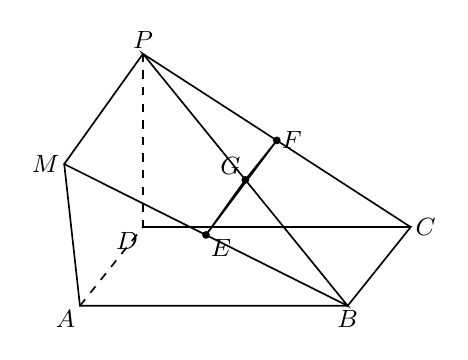
\begin{tikzpicture}[semithick, every node/.style={inner sep=1.5pt, font=\small}]
  \coordinate (A) at (0,0);
  \coordinate (B) at (3.4,0);
  \coordinate (C) at (4.2,1.0);
  \coordinate (D) at (0.8,1.0);
  \coordinate (M) at (-0.2,1.8);
  \coordinate (P) at (0.8,3.2);
  \coordinate (E) at (1.6,0.9);
  \coordinate (F) at (2.5,2.1);
  \coordinate (G) at (2.1,1.6);

  \draw (M) -- (A) -- (B) -- (C) -- (D);
  \draw (P) -- (M) -- (B) -- (P) -- (C);
  \draw[dashed] (P) -- (D);
  \draw[dashed] (A) -- (D);
  \draw (E) -- (F) -- (G) -- cycle;

  \fill (E) circle (1.4pt);
  \fill (F) circle (1.4pt);
  \fill (G) circle (1.4pt);
  \node[left] at (M) {$M$};
  \node[above] at (P) {$P$};
  \node[below left] at (A) {$A$};
  \node[below] at (B) {$B$};
  \node[right] at (C) {$C$};
  \node[below left] at (D) {$D$};
  \node[below right] at (E) {$E$};
  \node[right] at (F) {$F$};
  \node[above left] at (G) {$G$};
\end{tikzpicture}
\end{center}
\nopagebreak[4]
\Needspace{4\baselineskip}
\textbf{解析}

\Needspace{5\baselineskip}
以 $A$ 为原点，$AB$ 为 $x$ 轴，$AD$ 为 $y$ 轴，$AM$ 为 $z$ 轴建立空间直角坐标系。设 $MA=1$，则 $AD=PD=2$，故

\nopagebreak[4]
\[A(0,0,0),\ B(2,0,0),\ C(2,2,0),\ D(0,2,0),\]

\nopagebreak[4]
\[M(0,0,1),\ P(0,2,2).\]

\Needspace{5\baselineskip}
$E$，$F$，$G$ 分别为 $MB$，$PB$，$PC$ 的中点，故

\nopagebreak[4]
\[E\left(1,0,\frac12\right),\quad F(1,1,1),\quad G(1,2,1).\]

（1）平面 $PDC$ 经过 $P(0,2,2)$，$D(0,2,0)$，$C(2,2,0)$，三点 $y$ 坐标均为 $2$，故平面 $PDC$ 为 $y=2$，法向量可取 $\boldsymbol n_1=(0,1,0)$。

\Needspace{5\baselineskip}
平面 $EFG$ 中，

\nopagebreak[4]
\[\overrightarrow{FE}=\left(0,-1,-\frac12\right),\qquad \overrightarrow{FG}=(0,1,0).\]

\Needspace{5\baselineskip}
取法向量

\nopagebreak[4]
\[\boldsymbol n_2=\overrightarrow{FE}\times\overrightarrow{FG}
=\left(\frac12,0,0\right),\]

\Needspace{5\baselineskip}
即 $x$ 轴方向。因为 $\boldsymbol n_1\cdot\boldsymbol n_2=0$，所以两平面垂直，即

\nopagebreak[4]
\[\text{\text{平面} }EFG\perp\text{\text{平面} }PDC.\]

\Needspace{5\baselineskip}
（2）三棱锥 $P-MAB$ 的底面为 $\triangle MAB$，在 $y=0$ 平面内，

\nopagebreak[4]
\[S_{\triangle MAB}=\frac12\cdot AB\cdot MA=\frac12\times2\times1=1,\]

\Needspace{5\baselineskip}
$P$ 到平面 $MAB$ 的距离为 $2$，故

\nopagebreak[4]
\[V_{P-MAB}=\frac13\times1\times2=\frac23.\]

\Needspace{5\baselineskip}
四棱锥 $P-ABCD$ 的底面是边长为 $2$ 的正方形，面积为 $4$，高为 $P$ 到平面 $ABCD$（$z=0$）的距离 $2$，故

\nopagebreak[4]
\[V_{P-ABCD}=\frac13\times4\times2=\frac83.\]

\Needspace{5\baselineskip}
因此体积之比为

\nopagebreak[4]
\[\frac{V_{P-MAB}}{V_{P-ABCD}}=\frac{\frac23}{\frac83}=\frac14.\]

\gkanswer{答案：（1）证明；（2）$\dfrac14$。}

\end{answer}
\begin{answer}
\gksolhead{21}{}

\textbf{题目}：

已知函数 $f(x)=\ln x-ax+\dfrac{1-a}{x}-1$（$a\in\mathbf R$）。

（1）当 $a=-1$ 时，求曲线 $y=f(x)$ 在点 $(2,f(2))$ 处的切线方程；

（2）当 $a\leqslant\dfrac12$ 时，讨论 $f(x)$ 的单调性。

\Needspace{4\baselineskip}
\textbf{解析}

\Needspace{5\baselineskip}
（1）当 $a=-1$ 时，

\nopagebreak[4]
\[f(x)=\ln x+x+\frac2x-1,\]

\nopagebreak[4]
\[f'(x)=\frac1x+1-\frac2{x^2}.\]

\Needspace{5\baselineskip}
在 $x=2$ 处，

\nopagebreak[4]
\[f(2)=\ln2+2+1-1=\ln2+2,\qquad f'(2)=\frac12+1-\frac12=1.\]

\Needspace{5\baselineskip}
切线方程为

\nopagebreak[4]
\[y-(\ln2+2)=1\cdot(x-2),\]

\Needspace{5\baselineskip}
即

\nopagebreak[4]
\[y=x+\ln2.\]

\Needspace{5\baselineskip}
（2）函数定义域为 $(0,+\infty)$，且

\nopagebreak[4]
\[f'(x)=\frac1x-a-\frac{1-a}{x^2}
=\frac{-ax^2+x+a-1}{x^2}
=\frac{(x-1)(-ax+1-a)}{x^2}.\]

按 $a$ 分类讨论。

① 当 $a<0$ 或 $a=0$ 时，$-ax+1-a>0$ 对 $x>0$ 恒成立，故 $f'(x)$ 的符号由 $x-1$ 决定：

\begin{itemize}
\item $0<x<1$ 时 $f'(x)<0$，$f(x)$ 递减；
\item $x>1$ 时 $f'(x)>0$，$f(x)$ 递增。
\end{itemize}

② 当 $0<a<\dfrac12$ 时，令 $-ax+1-a=0$ 得 $x=\dfrac{1-a}{a}=\dfrac1a-1>1$。

\begin{itemize}
\item $0<x<1$ 时，$x-1<0$，$-ax+1-a>0$，故 $f'(x)<0$；
\item $1<x<\dfrac1a-1$ 时，$x-1>0$，$-ax+1-a>0$，故 $f'(x)>0$；
\item $x>\dfrac1a-1$ 时，$x-1>0$，$-ax+1-a<0$，故 $f'(x)<0$。
\end{itemize}

即 $f(x)$ 在 $(0,1)$ 与 $\left(\dfrac1a-1,+\infty\right)$ 上递减，在 $\left(1,\dfrac1a-1\right)$ 上递增。

\Needspace{5\baselineskip}
③ 当 $a=\dfrac12$ 时，

\nopagebreak[4]
\[f'(x)=\frac{(x-1)\left(1-\frac12x\right)}{x^2}
=-\frac{(x-1)^2}{2x^2}\leqslant0.\]

故 $f(x)$ 在 $(0,+\infty)$ 上单调递减（除 $x=1$ 处导数为 $0$）。

\gkanswer{答案：（1）$y=x+\ln2$；（2）$a<0$ 或 $a=0$ 时，减区间 $(0,1)$、增区间 $(1,+\infty)$；$0<a<\dfrac12$ 时，减区间 $(0,1)$ 与 $\left(\dfrac1a-1,+\infty\right)$，增区间 $\left(1,\dfrac1a-1\right)$；$a=\dfrac12$ 时在 $(0,+\infty)$ 上单调递减。}

\end{answer}
\begin{answer}
\gksolhead{22}{}

\textbf{题目}：

如图，已知椭圆 $\dfrac{x^2}{a^2}+\dfrac{y^2}{b^2}=1$（$a>b>0$）过点 $\left(1,\dfrac{\sqrt2}2\right)$，离心率为 $\dfrac{\sqrt2}2$，左、右焦点分别为 $F_1$、$F_2$。点 $P$ 为直线 $l:x+y=2$ 上且不在 $x$ 轴上的任意一点，直线 $PF_1$ 和 $PF_2$ 与椭圆的交点分别为 $A$、$B$ 和 $C$、$D$，$O$ 为坐标原点。

（1）求椭圆的标准方程；

（2）设直线 $PF_1$、$PF_2$ 的斜率分别为 $k_1$、$k_2$。

① 证明：$\dfrac1{k_1}-\dfrac3{k_2}=2$；

② 问直线 $l$ 上是否存在点 $P$，使得直线 $OA$、$OB$、$OC$、$OD$ 的斜率 $k_{OA}$、$k_{OB}$、$k_{OC}$、$k_{OD}$ 满足 $k_{OA}+k_{OB}+k_{OC}+k_{OD}=0$？若存在，求出所有满足条件的点 $P$ 的坐标；若不存在，说明理由。
\nopagebreak[4]
\begin{center}% 2010 年山东卷文科第 22 题：椭圆、直线 l 与点 P。
% 来源 PDF：普通高考/2010/2010山东文.pdf，SHA-256 95a69b861a29ca594f9118c9643efcdfd04cae3c4f374ff9fa009f7ac99712f4。
% 原页：第 2 页（A3 三栏）第 3 栏上部，书页码 622。
% 重绘依据：椭圆 x^2/2+y^2=1，F1(-1,0)、F2(1,0)；l:x+y=2；
%   P(0.4,1.6) 在 l 上，PF1 交椭圆于 A、B，PF2 交椭圆于 C、D。
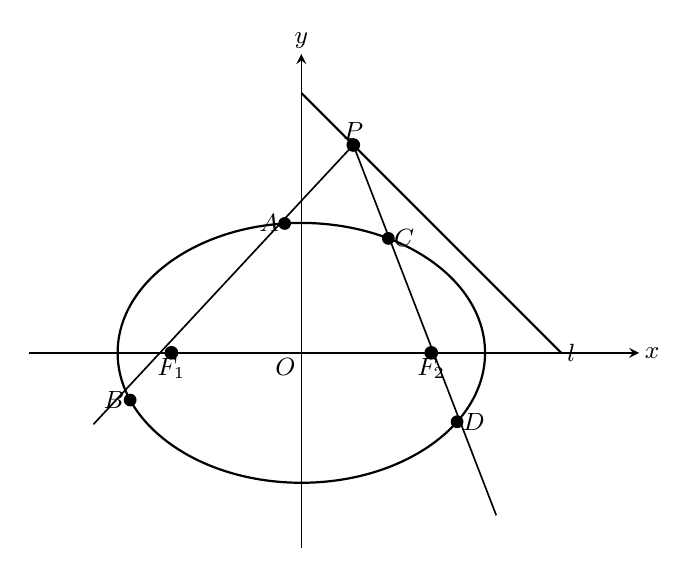
\begin{tikzpicture}[semithick, scale=1.65, every node/.style={inner sep=1.8pt, font=\small}]
  \draw[-stealth] (-2.1,0) -- (2.6,0) node[right] {$x$};
  \draw[-stealth] (0,-1.5) -- (0,2.3) node[above] {$y$};
  \draw[thick] (0,0) ellipse (1.414 and 1);
  \draw[thick] (0,2) -- (2,0) node[right] {$l$};
  \fill (-1,0) circle (1.5pt) node[below] {$F_1$};
  \fill (1,0) circle (1.5pt) node[below] {$F_2$};
  \fill (0.4,1.6) circle (1.5pt) node[above] {$P$};
  \draw (0.4,1.6) -- (-1.6,-0.55);
  \draw (0.4,1.6) -- (1.5,-1.25);
  \fill (-0.1286,0.9959) circle (1.4pt) node[left] {$A$};
  \fill (-1.3177,-0.3631) circle (1.4pt) node[left] {$B$};
  \fill (0.6697,0.8808) circle (1.4pt) node[right] {$C$};
  \fill (1.1989,-0.5304) circle (1.4pt) node[right] {$D$};
  \node[below left] at (0,0) {$O$};
\end{tikzpicture}
\end{center}
\nopagebreak[4]
\Needspace{4\baselineskip}
\textbf{解析}

\Needspace{5\baselineskip}
（1）由 $e=\dfrac{\sqrt2}2$ 得

\nopagebreak[4]
\[b^2=a^2(1-e^2)=a^2\left(1-\frac12\right)=\frac{a^2}2.\]

\Needspace{5\baselineskip}
椭圆过点 $\left(1,\dfrac{\sqrt2}2\right)$：

\nopagebreak[4]
\[\frac1{a^2}+\frac{\frac12}{b^2}=1
\iff \frac1{a^2}+\frac1{a^2}=1
\iff a^2=2.\]

\Needspace{5\baselineskip}
故 $b^2=1$，椭圆方程为

\nopagebreak[4]
\[\frac{x^2}{2}+y^2=1.\]

（2）由（1）$c=\sqrt{a^2-b^2}=1$，故 $F_1(-1,0)$，$F_2(1,0)$。

\Needspace{5\baselineskip}
设 $P(t,2-t)$，$t\neq2$（$P$ 不在 $x$ 轴上）。则

\nopagebreak[4]
\[k_1=\frac{2-t}{t+1},\qquad k_2=\frac{2-t}{t-1}.\]

\Needspace{5\baselineskip}
① 计算：

\nopagebreak[4]
\[\frac1{k_1}-\frac3{k_2}
=\frac{t+1}{2-t}-\frac{3(t-1)}{2-t}
=\frac{t+1-3t+3}{2-t}
=\frac{4-2t}{2-t}=2.\]

② 先求过焦点且斜率为 $k$ 的直线与椭圆两交点 $M$，$N$ 的斜率 $k_{OM}+k_{ON}$。

\Needspace{5\baselineskip}
\textbf{过 $F_1(-1,0)$ 时}，直线 $y=k(x+1)$，代入 $x^2/2+y^2=1$：

\nopagebreak[4]
\[\left(\frac12+k^2\right)x^2+2k^2x+k^2-1=0.\]

\Needspace{5\baselineskip}
设交点横坐标为 $x_1$，$x_2$，则

\nopagebreak[4]
\[x_1+x_2=-\frac{2k^2}{\frac12+k^2},\qquad x_1x_2=\frac{k^2-1}{\frac12+k^2}.\]

\Needspace{5\baselineskip}
而 $y_i=k(x_i+1)$，故

\nopagebreak[4]
\[k_{OM}+k_{ON}=\sum_{i=1}^2\frac{y_i}{x_i}
=k\left(2+\frac{x_1+x_2}{x_1x_2}\right)
=k\left(2-\frac{2k^2}{k^2-1}\right)
=\frac{2k}{1-k^2}.\]

\Needspace{5\baselineskip}
\textbf{过 $F_2(1,0)$ 时}，直线 $y=k(x-1)$，同理可得

\nopagebreak[4]
\[k_{OM}+k_{ON}=\frac{2k}{1-k^2}.\]

（两种情形公式相同，可直接代入验证。）

\Needspace{5\baselineskip}
于是题设

\nopagebreak[4]
\[k_{OA}+k_{OB}+k_{OC}+k_{OD}=0\]

\Needspace{5\baselineskip}
等价于

\nopagebreak[4]
\[\frac{2k_1}{1-k_1^2}+\frac{2k_2}{1-k_2^2}=0,\]

\Needspace{5\baselineskip}
即

\nopagebreak[4]
\[k_1(1-k_2^2)+k_2(1-k_1^2)=0
\iff (k_1+k_2)(1-k_1k_2)=0.\]

由①，$k_1=\dfrac{k_2}{2k_2+3}$。分两种情形：

\Needspace{5\baselineskip}
\textbf{情形一：$k_1+k_2=0$。} 则

\nopagebreak[4]
\[\frac{k_2}{2k_2+3}=-k_2
\iff k_2=0\text{ \text{或} }k_2=-2.\]

$k_2=0$ 使 $P$ 在 $x$ 轴上，舍去。$k_2=-2$ 时 $k_1=2$，由 $k_2=\dfrac{2-t}{t-1}=-2$ 得 $t=0$，故 $P(0,2)$。

\Needspace{5\baselineskip}
\textbf{情形二：$k_1k_2=1$。} 则

\nopagebreak[4]
\[\frac{k_2^2}{2k_2+3}=1
\iff k_2^2-2k_2-3=0
\iff k_2=3\text{ \text{或} }k_2=-1.\]

$k_2=3$ 时 $k_1=\dfrac13$，由 $\dfrac{2-t}{t-1}=3$ 得 $t=\dfrac54$，故 $P\left(\dfrac54,\dfrac34\right)$。

$k_2=-1$ 时 $k_1=-1$，此时 $PF_1$ 与 $PF_2$ 平行，不存在满足条件的有限点 $P$，舍去。

\Needspace{5\baselineskip}
综上，满足条件的点 $P$ 为

\nopagebreak[4]
\[P(0,2)\quad\text{\text{或}}\quad P\left(\frac54,\frac34\right).\]

\gkanswer{答案：（1）$\dfrac{x^2}{2}+y^2=1$；（2）① 证明，② $P(0,2)$ 或 $P\left(\dfrac54,\dfrac34\right)$。}

\end{answer}